\chapter{Web semântica}


\section{O que é Web Semântica\?}

A ideia de Web Semântica surgiu em 2001, após a publicação de um artigo através da revista \emph{Scientific American, denominado: The semantic Web: a new form of Web content that is meaningful to computers will unleash a revolution of new possibilities} (Web Semântica: um novo formato de conteúdo para a Web que tem significado para computadores vai iniciar uma revolução de novas possibilidades.”. Este artigo foi elaborado por Tim Berners-Lee, James Hendler e Ora Lassila \cite{intwebsem}.

Para que possamos entende-la melhor, precisamos compreender como funciona a Web\footnote{Web - \emph{World Wide Web} (em inglês). É sistema hipertextual que opera através da Internet.} atual e como ela chegou no que é hoje.

No início da internet, as páginas eram desenvolvidas por programadores de \emph{software} \cite{kbreitman}. Essas páginas eram feitas exclusivamente para apresentação da informação, ou seja, o processo de interpretação ficava todo a cargo dos seres humanos.

Com o passar dos anos, a internet foi ficando cada vez mais popular. De acordo com o site\emph{ internet live stats} \cite{totalwebsite}, no final de 2014, a web contará com aproximadamente 1 bilhão de \emph{websites}.

\graphicspath{{figuras/}}
\begin{figure}[H]
\centering
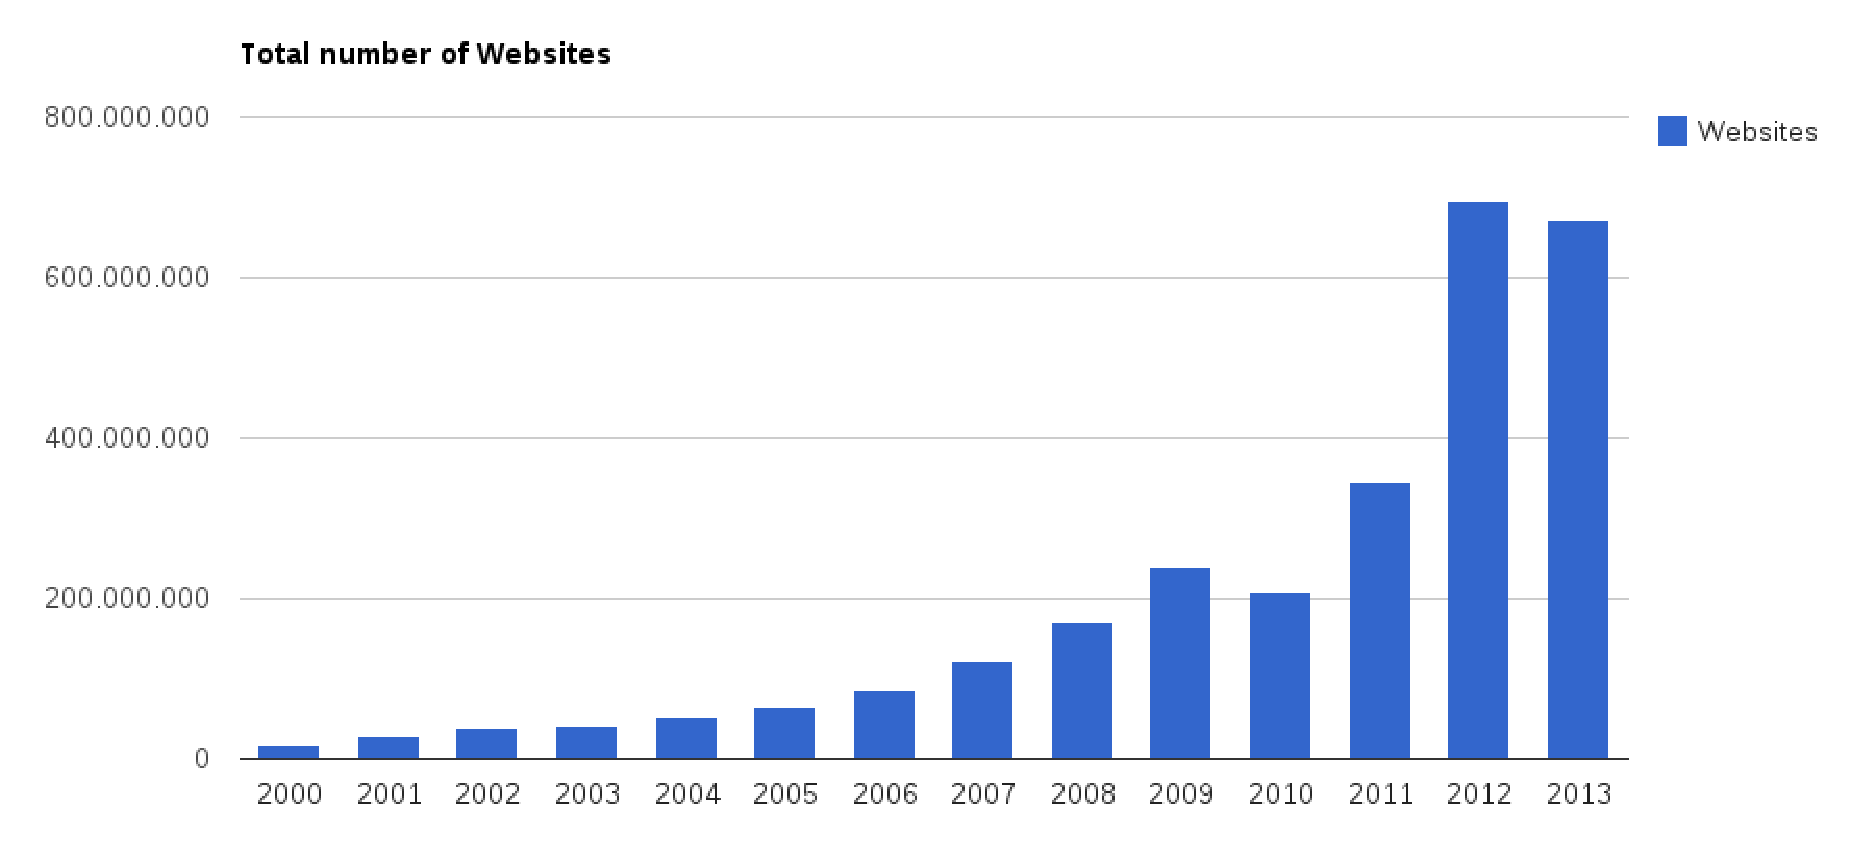
\includegraphics[width=0.9\textwidth]{numero_de_websites}
\caption[Número total de Websites por ano.]{Número total de \emph{Websites} por ano. Extraído de \cite{totalwebsite} }
\label{num-website}
\end{figure}

O grande problema desse avanço é que a maioria dos \emph{Websites} criados ainda mantém sua característica inicial, ou seja, ainda são feitos para as pessoas interpretarem  e não as máquinas. De acordo com a Karin Breitman \cite{kbreitman}, essa Web atual pode ser definida como Web Sintática.

Segue um exemplo para que possamos entender melhor esse conceito: vamos supor que você esteja pensando em tirar umas férias. Você deseja visitar um lugar quente e tropical e reservou um orçamento de 3.000 reais para a sua viagem. Você deseja ficar em um bom lugar, mas não quer que isso custe muito em seu orçamento. Você também quer fazer um bom negócio com as passagens de avião \cite{web3}. 

Com os recursos da  Web (sintática) que temos atualmente, nós teríamos que pesquisar bastante para encontrarmos a melhor opção. Teríamos que visitar vários sites de passagens aéreas e de hotéis e ainda comparar os preços entre eles. Seria um processo muito trabalhoso.

Em \cite{kbreitman}, são enumerados os maiores problemas que temos com os atuais mecanismos de busca na Internet, através de ferramentas do tipo \emph{Google\footnote{Google - Disponível em: \url{https://www.google.com.br/} }}, \emph{Yahoo\footnote{Yahoo - Disponívem em: \url{https://br.yahoo.com/}}} e \emph{Bing\footnote{Bing - Disponível em: \url{https://www.bing.com/}}}, por exemplo, como se segue:

\begin{itemize}
\item Grande numero de páginas encontradas, porém com pouca precisão – Por exemplo, ao realizar uma busca por TCP/IP no \emph{Google}, temos aproximadamente 14.900.000 resultados. Mesmo encontrando páginas relevantes, esse resultado seria de pouca utilidade caso a maioria das páginas fossem de pouca relevância.
\item Resultados são muitos sensíveis ao vocabulário – em determinados casos, até a ordem em que as palavras são digitadas tem impacto nos resultados. Muitas vezes os documentos relevantes acabam usando terminologias diferente das nossas.
\item Resultados são páginas individuais – em muitos casos temos um grande número de páginas no resultado que pertencem a um mesmo site. Seria mais interessante ter algum tipo de organização geográfica dos resultados. Ao final, temos de extrair manualmente as porções desses documentos de interesse.
\end{itemize}

\graphicspath{{figuras/}}
\begin{figure}[H]
\centering
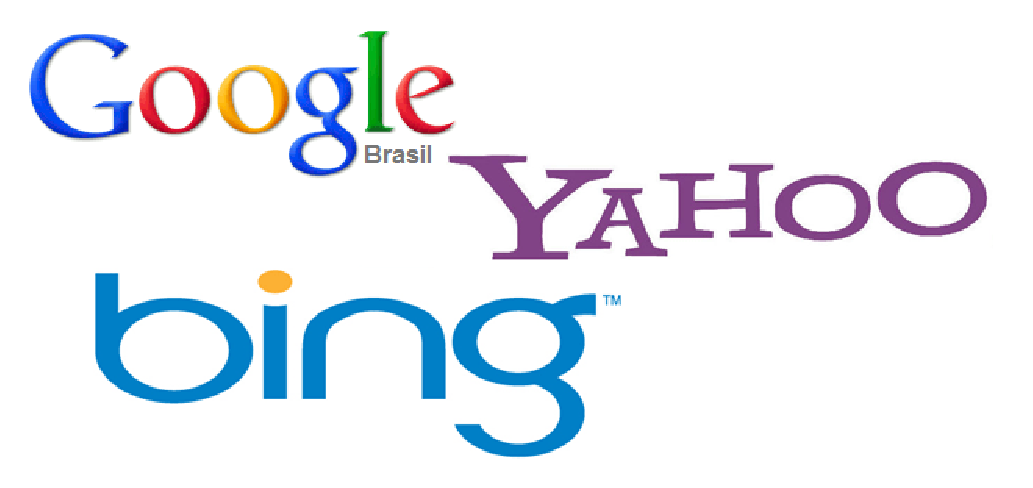
\includegraphics[width=0.7\textwidth]{Buscadores}
\caption[Buscadores web – principais meios de localização de informação.]{Buscadores web – principais meios de localização de informação. Extraído de \cite{intwebsem} }
\label{buscadores}
\end{figure}
O que podemos concluir dessas situações citadas acima, é que a Internet se tornou um meio para se compartilhar documentos entre pessoas, ao invés de ser um meio em que a troca de dados e informações pudessem ser processadas automaticamente.

No meio desse caos , Tim Berners-Lee, considerado por muitos o criador da Internet, apostou no aparecimento de uma Web mais organizada, mais conectada. Ele a chamou de Web Semântica.

De acordo com Bernes-Lee, Hendler e Lassila: “A Web Semântica é uma extensão da Web atual, na qual é dada à informação um significado bem definido, permitindo que computadores e pessoas trabalhem em cooperação”.

A ideia central é encontrar uma maneira de categorizar o conteúdo da Web de forma padronizada, facilitando seu acesso \cite{kbreitman}. A Web Semântica não se trata de uma nova rede de informações, mas sim de um projeto para aplicar conceitos inteligentes na internet atual. Nela cada informação vem com um significado bem definido e não se encontra mais solta no mar de conteúdo, permitindo uma melhor interação com o usuário.\cite{websemtecmundo}.


\section{Arquitetura da Web Semântica}

Não sabemos ainda como a web semântica será efetivamente construída, mas já existe uma arquitetura definida pela W3C (\emph{World Wide Web Consortium}). Segue abaixo sua representação:

\graphicspath{{figuras/}}
\begin{figure}[H]
\centering
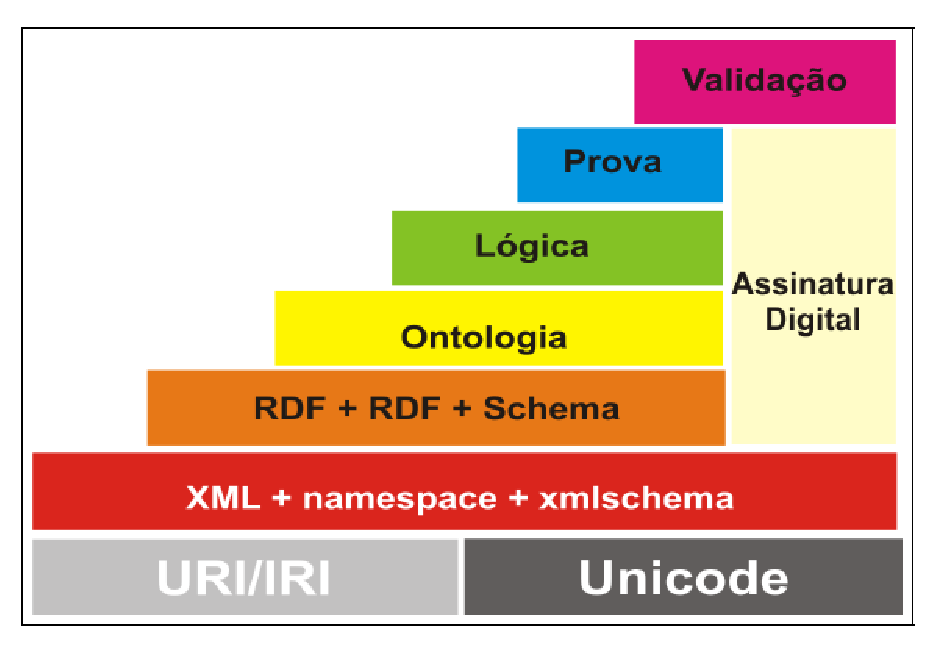
\includegraphics[width=0.8\textwidth]{arquitetura_web_semantica}
\caption[Arquitetura da Web Semântica.]{Arquitetura da Web Semântica. Extraído de \cite{fig-arqweb}}
\label{arq_web_sem}
\end{figure}

Como podemos perceber, a arquitetura da web semântica é formada por 7 camadas, cada uma com uma ferramenta e tecnologia diferente (ALVES, 2003). Tim Berners-Lee, definiu uma estrutura em camadas que reflete os passos que devem ser dados para que o projeto da Web Semântica seja realizado de uma forma incremental \cite{ferneda}. As próximas seções falaram um pouco sobre essas sete camadas.

\subsection{URI/IRI e UNICODE}

Vamos realizar uma abordagem \emph{bottom-up}(nota rodape), ou seja, vamos começar a análise pela camada mais inferior. Esta camada é composta pela URI (\emph{Uniform Resource Identifier}) e UNICODE que são padrões para a descrição e estabelecimento de identificadores universais do recurso e códigos internacionais de dados \cite{santarem}. Esses dois elementos são responsáveis pela designação de uma identificação mínima dos recursos na rede \cite{vesu}.

Segundo \cite{elementoswebsem}, o URI é um padrão para identificar um recurso físico ou abstrato de maneira única e global. Ele estabelece uma forma padrão para a identificação de recursos. Através da utilização de URI faz-se a referência para recursos representados na Web Semântica. No contexto da Internet, o conceito de URI já é bem utilizado. Na Web é utilizado um tipo de URI chamado URL. Através da URL é possível endereçar documentos utilizando protocolos específicos da Internet como http e ftp \cite{rosa}.

Já o UNICODE, de acordo com \cite{rosa}, é uma linguagem que define uma forma padrão para a representação de caracteres. Unicode proporciona uma forma única para a representação de um caractere não importando a plataforma, o programa nem a linguagem que está sendo utilizada. A utilização de Unicode na Web Semântica proporciona a capacidade de troca de símbolos de maneira universal, requisito fundamental para o sucesso desta nova proposta de representação de informação na Internet. 

\subsection{XML, NAMESPACE e XML Schema}

Essa camada 2, também chamada de camada sintática, é responsável pelo estabelecimento correto da sintaxe de descrição dos dados.

O XML é uma linguagem de marcação que, diferentemente do HTML, permite a criação e o uso de tags personalizadas, fornecendo assim uma maneira simples de organizar e estruturar os dados existentes em uma determinada aplicação \cite{XML2009}. Atualmente, o XML é a linguagem padrão recomendada pelo W3C\footnote{W3C - Disoinível em: \url{http://www.w3c.br/Home/WebHome}} para troca de dados via Web.

Hoje, a Web Semântica exige uma descrição formal da semântica dos dados, de tal forma a evitar ambiguidades e permitir a interpretação de informações por parte das aplicações. Neste contexto, XML provê uma sintaxe bem definida, sendo atualmente utilizado na maioria das aplicações existentes na Web \cite{filholoscio}.

\graphicspath{{figuras/}}
\begin{figure}[H]
\centering
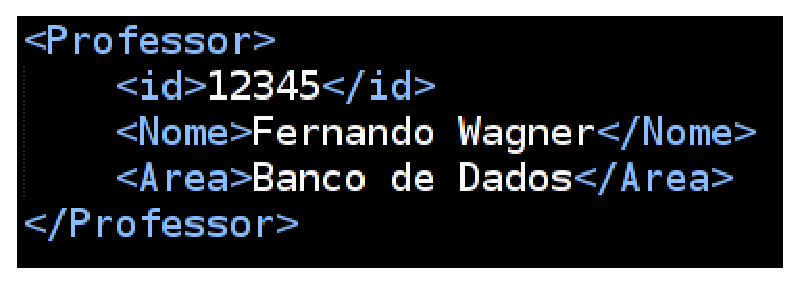
\includegraphics[width=0.6\textwidth]{xml1}
\caption{Trecho de código XML destacando dados de um professor.}
\label{xml1}
\end{figure}

\graphicspath{{figuras/}}
\begin{figure}[H]
\centering
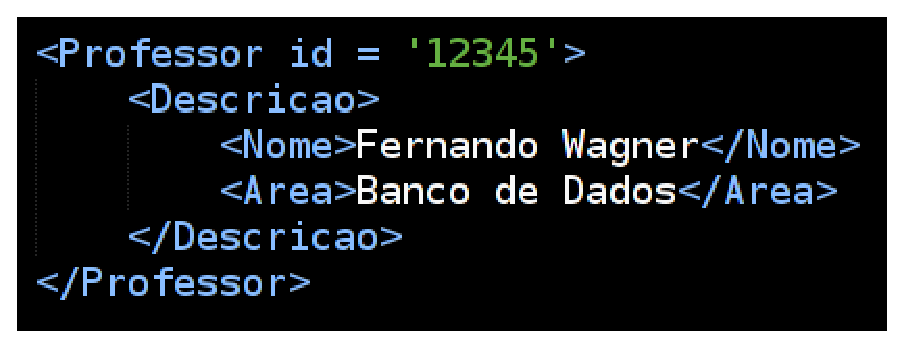
\includegraphics[width=0.6\textwidth]{xml2}
\caption{Documento XML alternativo ao da figura \ref{xml1}.}
\label{xml2}
\end{figure}

Um fato importante a ser levado em consideração no XML, é que um mesmo conjunto de dados podem ser representados de várias formas. Se observarmos figura \ref{xml2}, por exemplo, podemos perceber que ela é uma versão alternativa a figura \ref{xml1}. Essa característica pode causar algumas discordâncias entre aplicações. 

Para contornar esses problemas, foram criadas linguagens que definem esquemas para XML. São uma espécie de contrato, onde todas as partes envolvidas por um contexto de aplicação devem escrever seus documentos XML seguindo o padrão de estruturação especificado no esquema XML correspondente. Dentre as linguagens para definição de esquemas XML, destacam-se DTD\footnote{DTD - \emph{Document Type Definition}. Disponível em: \url{http://www.w3schools.com/DTD/}} e XML Schema \cite{filholoscio}.

De acordo com \cite{rosa}, XML Schema é uma ferramenta que permite a definição e a descrição de estruturas e de conteúdos de documentos XML. Através dessa linguagem, define-se o formato válido de um documento XML, incluindo quais elementos e atributos são permitidos ou não, quais são as suas localizações, o número de ocorrências de cada elemento e outras características, Ou seja, proporciona mecanismos para a definição de gramáticas para correção de documentos XML.

O último elemento dessa camada, são os chamados \emph{namespaces}. Eles são classificados como um método para qualificar nomes de elementos e atributos usados em documentos XML, através da associação de referências URI. Através desse mecanismo de espaço de nomes, é possível a combinação de documentos com a utilização de vocabulário compartilhado. Através do mecanismo de espaço de nomes definido em XML, é possível compartilhar e reutilizar a definição de outros esquemas XML sem que haja problemas de colisão de nomes \cite{rosa} .

\subsection{RDF e RDF Schema}

Essa camada também pode ser chamada de camada de dados. Ela está diretamente relacionada com a representação, o processamento e a codificação dos metadados \cite{vesu}. Para isso estão presentes nessa camada a arquitetura de metadados RDF e o RDF Schema, que são ferramentas responsáveis por expressar significados e promover a interoperabilidade entre metadados e padrões ou formatos de metadados \cite{santarem}.

Segundo Rosa \cite{rosa}, RDF (\emph{Resource Description Framework}) é uma linguagem para representação de informação na Web. Trata-se de uma infra-estrutura que fornece a habilidade para codificação, troca e reutilização de metadados. RDF define um modelo de dados para descrição de semântica de dados para o entendimento do computador. É o fundamento para o processamento de metadados (informação sobre informação). 

O RDF veio como uma alternativa para o XML, que mesmo sendo recomendado pelo W3C e amplamente utilizado em aplicações, tinha muitas limitações para descrever adequadamente a semântica de uma informação. Com o RDF, conseguimos expressar como os elementos devem se relacionar.

Como já foi dito, o RDF é um modelo de dados. Esse modelo possibilita a definição de afirmações, chamadas sentenças, sobre um recurso.

De acordo com \cite{filholoscio}, Entende-se por um recurso, “qualquer coisa” sobre a qual se quer expressar uma ideia. Um recurso pode estar relacionado com dados ou com outros recursos através das sentenças. Uma sentença é estruturada no formato sujeito + predicado + objeto onde: 

\begin{itemize}
\item Sujeito: Tem como valor o recurso do qual se quer escrever uma sentença.
\item Predicado: Especifica um relacionamento entre sujeito e objeto. O predicado é especificado através de propriedades, que são relações binárias, geralmente nomeadas por um verbo e permitem relacionar um recurso a dados ou a outros recursos. 
\item Objeto: Denomina o recurso ou dado que se relaciona ao sujeito.

\end{itemize}

Por causa de seu formato, uma sentença também é chamada de Tripla. Logo, um documento de RDF pode ser visto como um conjunto de triplas que descrevem informações sobre recursos de um certo domínio. Abaixo, vemos uma forma abstrata de representar essas triplas:

\graphicspath{{figuras/}}
\begin{figure}[H]
	\centering
	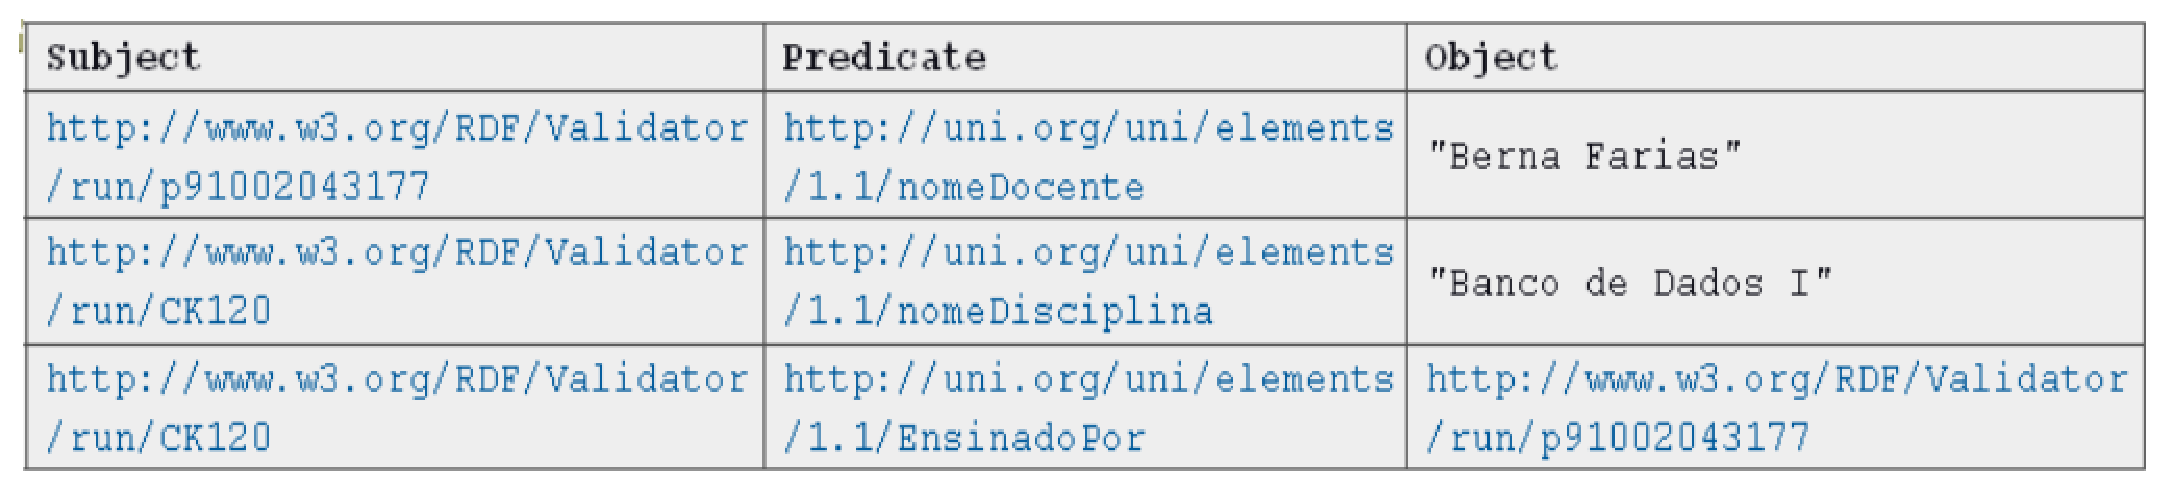
\includegraphics[width=1.0\textwidth]{tripla_rdf}
	\caption[Forma abstrata de visualizar triplas.]{Forma abstrata de visualizar triplas. Extraído de \cite{filholoscio}}
	\label{tripla_rdf}
\end{figure}

Realizando uma breve análise da figura \ref{tripla_rdf}, percebemos que ela é composta por dois recursos: “p91002043177” e “CK120”.

Na primeira tripa, temos o recurso “p91002043177” recebendo o nome “Berna Farias”.

Na segunda, o recurso “CK120” recebe o nome “Banco de Dados”.

E na terceira tripla, temos a descrição de um relacionamento entre os dois recursos. Essa Relação foi criada através do predicado “EnsinadoPor”.

Uma outra forma de representação muito utilizada é a de grafos. Esses grafos são compostos de nós e arcos, que representam os recursos, suas propriedades e valores. Abaixo, é mostrado uma representação de um grafo da figura \ref{tripla_rdf}.

\graphicspath{{figuras/}}
\begin{figure}[H]
	\centering
	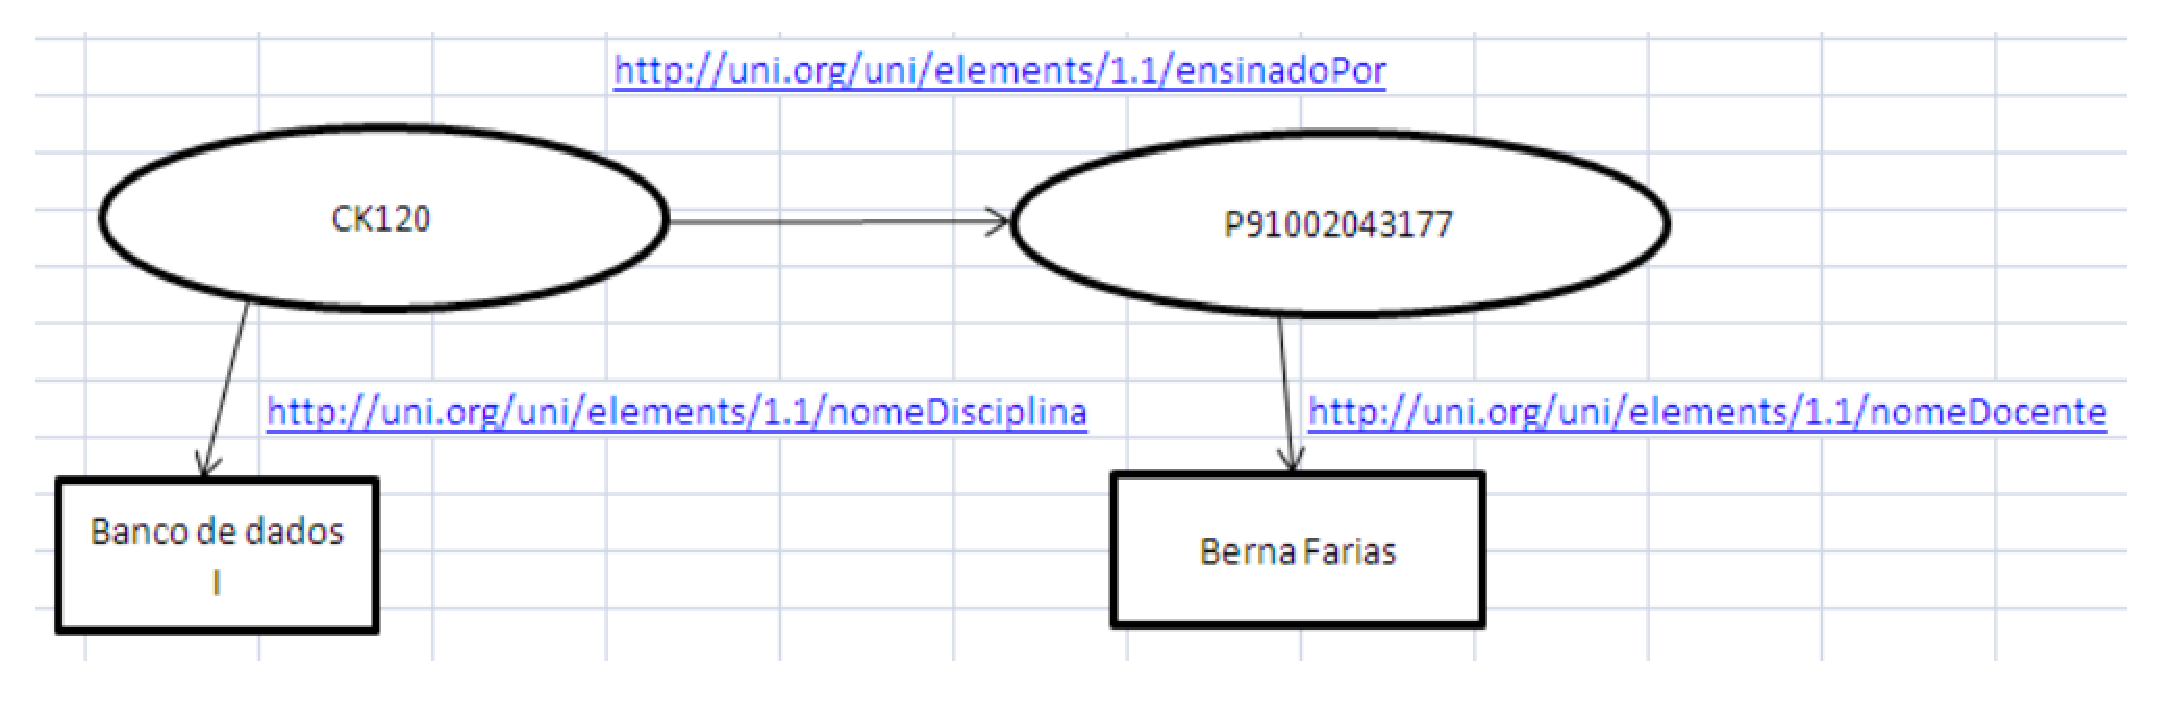
\includegraphics[width=1.0\textwidth]{grafo_rdf}
	\caption[Visualização de triplas através de um grafo.]{Visualização de triplas através de um grafo. Extraído de \cite{filholoscio}}
	\label{grafo_rdf}
\end{figure}

Na figura \ref{grafo_rdf}, Os chamados Nós literais são representados pelas caixas e os Nós referência são representados pelas URIs nas elipses. 

Para Conseguimos uma certa compatibilidade entre a escrita e os grafos RDFs, foi criada uma linguagem chamada RDF/XML. Com isso, um documento escrito em RDF pode ser facilmente transformado em um grafo caso ele siga a sintaxe da linguagem. Abaixo, segue uma representação do grafo em uma linguagem com base em XML:

\graphicspath{{figuras/}}
\begin{figure}[H]
	\centering
	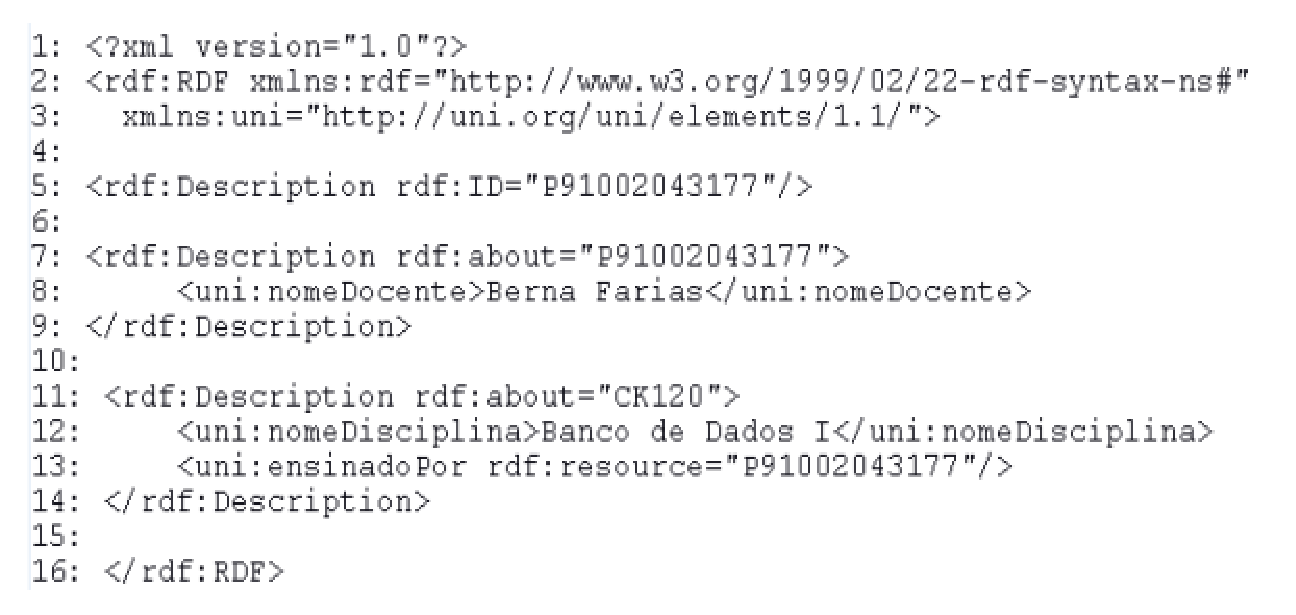
\includegraphics[width=1.0\textwidth]{rdf_xml}
	\caption[Trecho de um documento RDF que representa o grafo da figura \ref{grafo_rdf}. ]{Trecho de um documento RDF que representa o grafo da figura \ref{grafo_rdf} . Extraído de \cite{filholoscio}}
	\label{rdf_xml}
\end{figure}

O RDF Schema tem uma função parecida com o XML Schema da seção anterior. De acordo com \cite{rosa}: é uma linguagem que define a estrutura válida para dos documentos RDF. RDF e RDF Schema são recomendações do consórcio W3C que definem o padrão para a representação de metadados. São a base de todas as linguagens para expressar semântica da Web Semântica, devido à adoção pelo consórcio W3C.
	
Portanto, considerando que o RDF pode conter inconsistências, o RDFS visa solucionar tais problemas provendo construtores que permitem especificar formalmente um esquema \cite{filholoscio}. O estratégia é pra funcionar da seguinte forma: todas as sentenças descritas num documento RDF deverá obedecer à semântica descrita no esquema RDFS, onde esse esquema nada mais é que a modelagem do domínio de interesse.

\subsection{Ontologia}

O RDF conseguiu suprir algumas deficiências do XML em relação a semântica de dados, mas comparado a ontologias ele se torna bastante limitado. Ele basicamente serve para escrever sentenças sem que haja qualquer descrição formal de um domínio \cite{filholoscio}. As ontologias surgiram para suprir algumas características que o RDF não contempla. De acordo com \cite{filholoscio}, são algumas dessas características:

\begin{itemize}

\item Restrições de propriedades: Muitas vezes precisamos impor restrições nos valores que uma propriedade pode assumir. Por exemplo, não conseguimos dizer em RDF/RDFS que um time de futebol tem que ter, no mínimo, onze jogadores para poder disputar uma partida. 

\item Disjunção de classes: No domínio-alvo pode acontecer de classes (conceitos) serem disjuntos. Por exemplo, homem e mulher são dois conceitos disjuntos, pois uma pessoa não pode ser do sexo masculino e feminino ao mesmo tempo. Em RDF/RDFS, é possível somente expressar relações de hierarquia como mulher é subclasse de pessoa.

\item Combinação entre classes: RDF/RDFS não permite que se criem novos conceitos utilizando uma combinação de conceitos já especificados usando, por exemplo, a união ou interseção destes.  

\item Características de propriedades: Também não é possível especificar na camada de RDF/RDFS algumas características de propriedades como, por exemplo, a transitividade de valores.

\end{itemize}

Essa camada é importante, pois além de ter a definição dos significados e semântica dos dados é nela que estão estabelecidos os esquemas classificatórios utilizados pelos agentes de softwares \cite{santarem}. Vamos descreve-la melhor num outro capítulo.

\subsection{Lógica}

De acordo com \cite{rosa}, a camada de Lógica proporciona a definição de semântica em linguagem formal habilitando a execução de serviços inteligentes. É composta principalmente por regras de inferência, com as quais os agentes poderão se utilizar para relacionar e processar informação. 

Vamos a um exemplo extraído de \cite{ferneda}: imaginando que uma revendedora de veículos define que quem vender mais do que 20 produtos em um ano será categorizado como Super Vendedor. Um programa pode seguir essa regra e fazer uma simples dedução: “José vendeu 25 veículos, portanto José é um Super Vendedor”. 

Depois de definido um sistema que segue a lógica, ou seja, as regras de inferência, podemos construir a prova.

\subsection{Prova}

De acordo com \cite{rosa}: De posse das regras de inferência da camada imediatamente inferior a esta (camada de prova), os agentes podem ter mais poder para raciocinar sobre conceitos e relacioná-los na camada de ontologia. Esta é a camada na qual pode-se obter explicações (provas) sobre as respostas dadas por agentes que consomem alguma informação com o objetivo de verificar se a dedução foi correta.

Com essa camada, podemos relacionar vários conceitos de lógica processadas pelo agentes para a construção de prova.

Podemos citar um outro exemplo de \cite{ferneda} para entendermos melhor: os registros da empresa mostram que Maria vendeu 15 automóveis e 8 caminhões. O sistema define que automóveis e caminhões são produtos da empresa. As regras matemáticas dizem que 15 + 8 = 23, que é maior que 20. Existe uma regra que diz que quem vende mais de 20 produtos é classificado como Super Vendedor. O computador junta as regras para provar que Maria é uma Super Vendedora. 

\subsection{Validação}

Segundo \cite{santarem}, essa última camada da Web Semântica é responsável pelo estabelecimento de verdades, ou seja, pelo estabelecimento de autenticidade, confiabilidade e validade dos dados na Web Semântica.

Por causa dessas verdades, essa camada também é chamada de camada de confiança. De acordo com \cite{rosa}, A camada de confiança (\emph{Trust}) conjuntamente com a camada de assinatura digital (\emph{digital signature}) proporciona mecanismos para prevenção de inconsistências na Web Semântica. Através de aplicações criadas neste nível, é possível criar agentes que saibam dizer, identificar e validar algum tipo de informação. Trata-se de outra característica importante da Web Semântica e muito importante no ambiente da Internet, na qual blocos de dados encriptados podem ser utilizados para garantir a autenticidade das fontes e a confiabilidade da informação que os agentes consultam. 




